\documentclass[
orientation = landscape,
aspectratio = 149,
10pt, usenames,
]{beamer}
\mode<presentation>{
\setbeamercovered{transparent}
%\beamertemplatenavigationsymbolsempty
\setbeamertemplate{footline}[frame number]
% 	\usefonttheme{professionalfonts}
}

\author{RA}\subject{Talk}

% https://tex.stackexchange.com/questions/446063/change-background-colour-to-black-and-text-to-white
\usecolortheme{owl}



\usepackage{graphicx}
\graphicspath{{./images/}}
\AtBeginDocument{\DeclareGraphicsExtensions{.eps, .png, .gif, .pdf, .jpg}}

\usepackage[english]{babel}
\usepackage[T1]{fontenc}
\usepackage{times}

\usepackage{hyperref}
% \hypersetup{pdfpagemode=FullScreen}

% http://texdoc.net/texmf-dist/doc/fonts/dingbat/dingbat.pdf
%\usepackage{dingbat}
%\usepackage{bbding}

% % https://tex.stackexchange.com/questions/34604/entering-unicode-characters-in-latex
% \usepackage[utf8]{inputenc}

% % https://texblog.org/2013/10/01/rotate-an-image-table-or-paragraph-in-latex/
% \usepackage{rotating}

% https://tex.stackexchange.com/questions/132783/how-to-write-checkmark-in-latex
% http://tug.ctan.org/info/symbols/comprehensive/symbols-a4.pdf
\usepackage{pifont}

% Color names
\usepackage{xcolor}

% https://tex.stackexchange.com/questions/152392/date-format-yyyy-mm-dd
\usepackage{datetime2}


% https://tex.stackexchange.com/questions/34166/understanding-minipages-aligning-at-top
\usepackage{adjustbox}

% https://tex.stackexchange.com/questions/124256/how-do-i-get-numbered-entries-in-a-beamer-bibliography
\setbeamertemplate{bibliography item}{\insertbiblabel}

\setbeamersize{text margin left=10pt, text margin right=10pt}
\setbeamertemplate{itemize items}[circle]

\beamertemplatenavigationsymbolsempty


% http://tex.stackexchange.com/questions/8680/how-can-i-insert-a-newline-in-a-framebox
%\usepackage{minibox}
%\usepackage{framed}
%\usepackage[usestackEOL]{stackengine}

% https://tex.stackexchange.com/questions/433450/how-to-frame-any-environment-like-minipage-and-others
% \usepackage{framed}


%% % http://tex.stackexchange.com/questions/167000/annotating-tables-with-tikz-adding-arrows
%% \usepackage{color, colortbl}
\usepackage{tikz}
%\tikzstyle{every picture}+=[remember picture]
%\usetikzlibrary{tikzmark}
%%\usetikzlibrary{tikzmark, positioning, fit, shapes.misc}

% http://tex.stackexchange.com/questions/91124/itemize-removing-natural-indent
\usepackage{enumitem}
% https://tex.stackexchange.com/questions/13463/specifying-bullet-type-when-using-itemize/13466
% https://tex.stackexchange.com/questions/24371/does-enumitem-conflict-with-beamer-for-lists
\setitemize{label=\usebeamerfont*{itemize item}\usebeamercolor[fg]{itemize item}\usebeamertemplate{itemize item}}

%% http://tex.stackexchange.com/questions/41408/a-five-level-deep-list
%\usepackage{enumitem}
%\setlistdepth{9}

%% https://tex.stackexchange.com/questions/20792/how-to-superimpose-latex-on-a-picture
%\usepackage{overpic}

% % http://tex.stackexchange.com/questions/32661/how-to-locate-figures-with-x-y-specified-location-in-a-presentation
% \usepackage[absolute,overlay]{textpos} % absolute positioning of stuff
% \setlength{\TPHorizModule}{1mm}
% \setlength{\TPVertModule}{1mm}

%\usepackage[makeroom]{cancel}

% \usepackage{amssymb}
% \usepackage{nicefrac}
% \usepackage{bbm}
% \usepackage{esint}
% \usepackage{sidecap}


%% http://tex.stackexchange.com/questions/17611/how-does-one-type-chinese-in-latex
%\usepackage{CJKutf8}
%\AtBeginDvi{\input{zhwinfonts}}


\usepackage{listings}

\definecolor{codegreen}{rgb}{0,0.6,0}
\definecolor{codegray}{rgb}{0.5,0.5,0.5}
\definecolor{codepurple}{rgb}{0.58,0,0.82}
\definecolor{backcolour}{rgb}{0.95,0.95,0.92}

\lstdefinestyle{mystyle}{
%backgroundcolor=\color{backcolour},
otherkeywords={self,yield,True,False},
commentstyle=\color{codegreen},
keywordstyle=\color{magenta},
numberstyle=\tiny\color{codegray},
stringstyle=\color{codepurple},
basicstyle=\ttfamily\scriptsize\bfseries,
breakatwhitespace=false, breaklines=true,
captionpos=b, keepspaces=true, numbers=none, showspaces=false,
numbersep=5pt, showstringspaces=false, showtabs=false, tabsize=2,
}

\lstset{style=mystyle}


%%%%%%%%%%%%%%%%%%%%%%%%%%%%%%%%%%%%%%%%%%%%%%%%%%%%%%%%%%%%%%%%%%%%%%%%%%%%%%%%
%%%%%%%%%%%%%%%%%%%%%%%%%%%%%%%%%%%%%%%%%%%%%%%%%%%%%%%%%%%%%%%%%%%%%%%%%%%%%%%%

\newcommand{\skipline}{{\ }\\}

% https://tex.stackexchange.com/questions/53511/line-spacing-with-mixed-font-sizes-in-itemize-environment
\newcommand{\citeinline}[3]{{\colorlet{backup}{.}\footnotesize\begin{itemize}[topsep=0.1\baselineskip,after=\vspace{-0pt}]
	                                                              \item[\color{backup}{\raisebox{0.1\baselineskip}{$\star$}}]\color{backup}#1\color{backup}#2\color{backup}\textsc{(#3)}
\end{itemize}\par}}


% http://tex.stackexchange.com/questions/211518/beamer-vfill-and-itemize
\def\Bottom#1{\vskip 0pt plus 1filll #1}
\def\BottomRight#1{\Bottom{\hfill #1}}



\definecolor{SeeMeBarely}{RGB}{230,230,230}
\definecolor{Purple}{RGB}{128,0,128}
\definecolor{DeepPurple}{RGB}{32,0,96}
\definecolor{quote}{RGB}{0, 0, 130}
\definecolor{britishracinggreen}{rgb}{0.0, 0.26, 0.15}

\newcommand{\ra}[1]{{\color{blue}{#1}}}
\newcommand{\cred}[1]{{\color{red}{#1}}}
\newcommand{\cblu}[1]{{\color{blue}{#1}}}
\newcommand{\cpur}[1]{{\color{Purple}{#1}}}
\newcommand{\gray}[1]{{\color{gray}{#1}}}

% http://www.webnots.com/vibgyor-rainbow-color-codes/
\definecolor{a}{RGB}{148, 0, 211}
\definecolor{b}{RGB}{75, 0, 130}
\definecolor{c}{RGB}{0, 0, 255}
\definecolor{d}{RGB}{0, 160, 0}
\definecolor{e}{RGB}{200, 200, 0}
\definecolor{f}{RGB}{255, 127, 0}
\definecolor{g}{RGB}{255, 0, 0}
%
\definecolor{z}{RGB}{0, 0, 0}
\definecolor{w}{RGB}{255, 255, 255}


\newcommand{\citemainpaper}{{%
\citeinline{%
\color{britishracinggreen}
Improved ribosome-footprint and mRNA measurements
provide insight into dynamics and regulation
of yeast translation.
}{%
Weinberg DE, Shah P, Eichhorn SW,
Hussmann JA, Plotkin JB, Bartel DP.
}{%
Cell Rep, 2016%
}%
}}


%%%%%%%%%%%%%%%%%%%%%%%%%%%%%%%%%%%%%%%%%%%%%%%%%%%%%%%%%%%%%%%%%%%%%%%%%%%%%%%%
\begin{document}
%%%%%%%%%%%%%%%%%%%%%%%%%%%%%%%%%%%%%%%%%%%%%%%%%%%%%%%%%%%%%%%%%%%%%%%%%%%%%%%%
%%%%%%%%%%%%%%%%%%%%%%%%%%%%%%%%%%%%%%%%%%%%%%%%%%%%%%%%%%%%%%%%%%%%%%%%%%%%%%%%
	
	
	\begin{frame}[plain,t]{}{}
	{
	\tiny\color{lightgray}
	\hfill{\DTMnow}
	\par
	}
		
		\begin{center}
			\vspace{1cm}
			Humpy Dumpty
			\\
			\gray{Team03}
		
		\end{center}
		
		\Bottom{
		\scriptsize
		%
		Roman Andreev (andreevr \textsc{\tiny{cat}} ethz \textsc{\tiny{dog}} ch)
		\hfill
		2020-11
		\\[0.5\baselineskip]
		}
	\end{frame}


%%%%%%%%%%%%%%%%%%%%%%%%%%%%%%%%%%%%%%%%%%%%%%%%%%%%%%%%%%%%%%%%%%%%%%%%%%%%
%%%%%%%%%%%%%%%%%%%%%%%%%%%%%%%%%%%%%%%%%%%%%%%%%%%%%%%%%%%%%%%%%%%%%%%%%%%%
	
	
	\begin{frame}[plain,t]{Humpy Dumpy aligner -- workflow}{}
		\begin{minipage}[t]{0.75\textwidth}
			\vspace{0pt}
			
			{\ }
			
			\only<2->{
			python \textbf{humdum\_aligner.py} genome reads1 reads2
			\begin{itemize}
				\item
				generates/writes an index of the reference genome
				\item
				prints all reads in SAM format
				(forward to file with ``>'')
			\end{itemize}
			}
			
			\bigskip
			
			\only<3->{
			python \textbf{humdum\_qc.py} samfile
			\begin{itemize}
				\item
				coverage, transcript lengths, mapping quality
				
				\medskip
				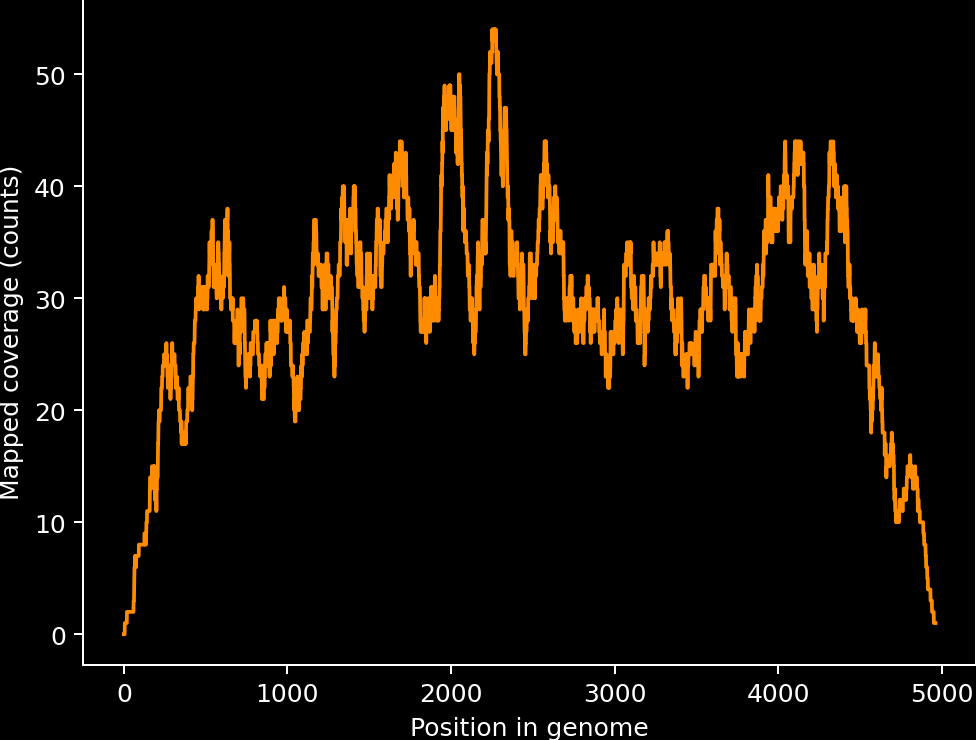
\includegraphics[width=0.3\textwidth]{coverage_small}
				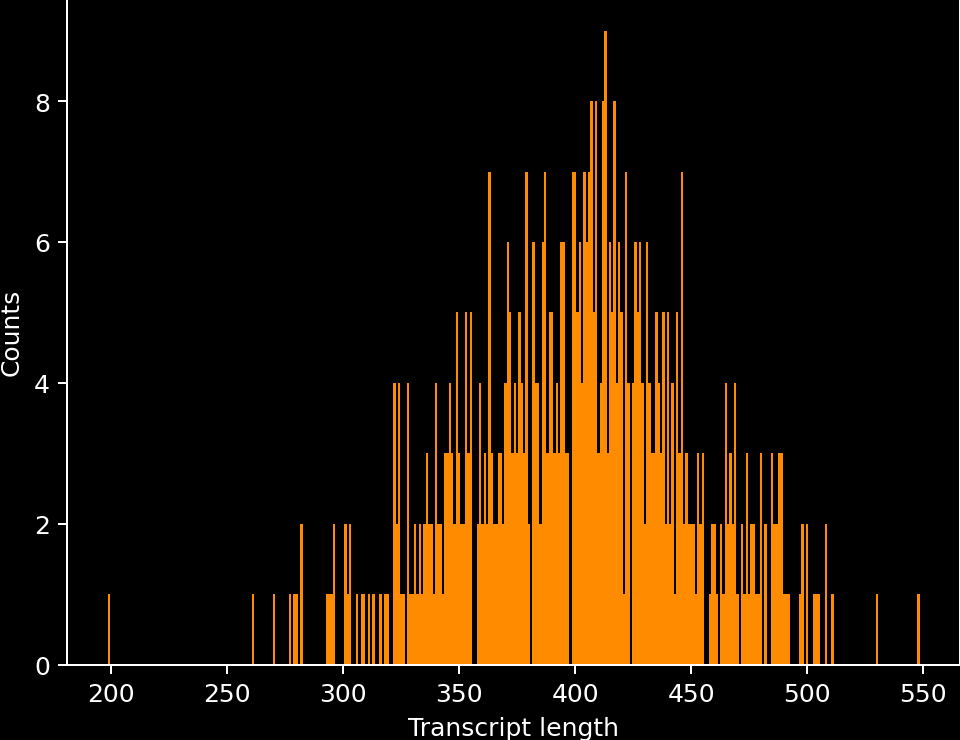
\includegraphics[width=0.3\textwidth]{tlenhist_small}
				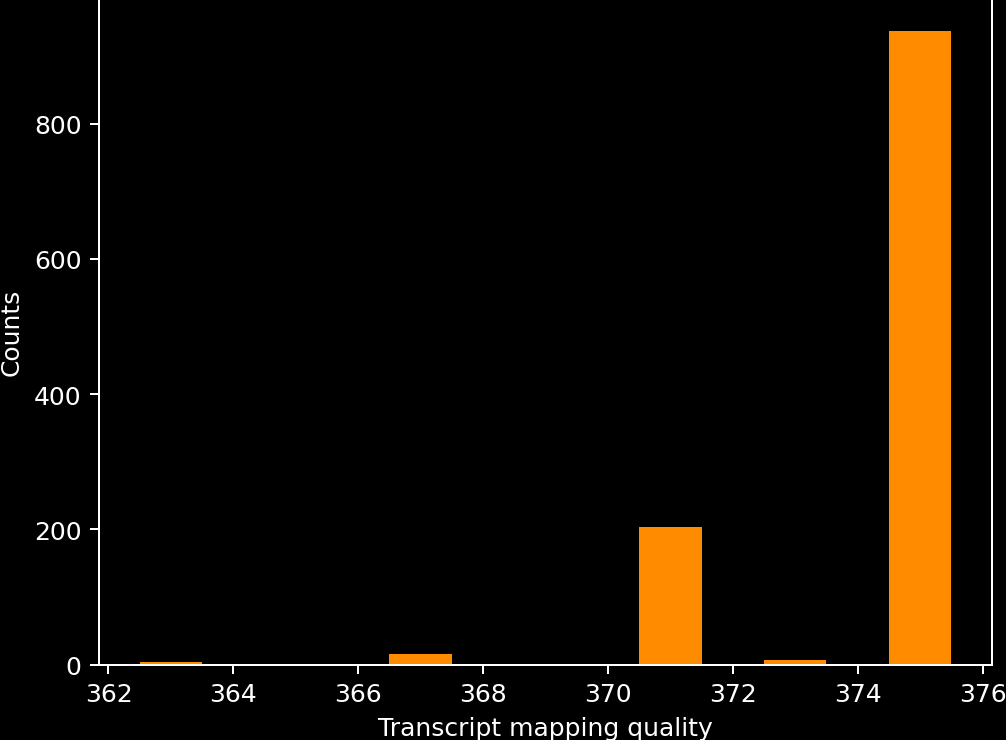
\includegraphics[width=0.3\textwidth]{mapqhist_small}
			\end{itemize}
			}

			\bigskip
			
			\only<4>{
			FM-Index: Luca
			\qquad
			S--W: Hendrik
			\qquad
			IO, QC, etc.: Roman
			}
		\end{minipage}
		%
		\begin{minipage}[t]{0.2\textwidth}
			\vspace{0pt}
			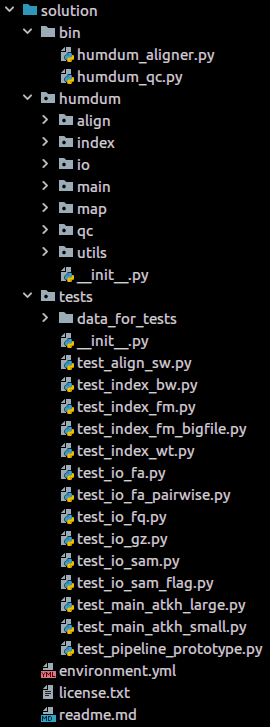
\includegraphics[height=0.85\textheight]{files}
		\end{minipage}
	\end{frame}
	
	%
	
	\begin{frame}[plain,t,fragile]{}{}
		\only<1>{
		\lstinputlisting[language=Python]{snippets/main.py}
		}
		\only<2>{
		\lstinputlisting[language=Python]{snippets/map_paired.py}
		}
		\only<3>{
		\lstinputlisting[language=Python]{snippets/map_one.py}
		}
		\only<4>{
		\lstinputlisting[language=Python]{snippets/map_pair.py}
		}
		
		\vspace{-5\baselineskip}
	\end{frame}

%
%%
%
%\begin{frame}[t]{}{}
%\end{frame}
%
%%
%
%\begin{frame}[t]{}{}
%\end{frame}


%%%%%%%%%%%%%%%%%%%%%%%%%%%%%%%%%%%%%%%%%%%%%%%%%%%%%%%%%%%%%%%%%%%%%%%%%%%%%%%%%
%\section{Extra}
%%%%%%%%%%%%%%%%%%%%%%%%%%%%%%%%%%%%%%%%%%%%%%%%%%%%%%%%%%%%%%%%%%%%%%%%%%%%%%%%%
%
%
	\newcounter{finalframe}
	\setcounter{finalframe}{\value{framenumber}}
% Backup frames follow
%
%
% \begin{frame}
% 	Appendix
% \end{frame}
%
%%
%
%\begin{frame}
%	%
%\end{frame}
%
	
	\setbeamercolor{background canvas}{bg=black}
	\begin{frame}[plain,b]
		\hfill
		\tiny
		\color{gray}
		this slide is intentionally left blank
	\end{frame}
	\setbeamercolor{background canvas}{bg=white}

%
	
	\begin{frame}[plain]{}{}
	\end{frame}


%%%%%%%%%%%%%%%%%%%%%%%%%%%%%%%%%%%%%%%%%%%%%%%%%%%%%%%%%%%%%%%%%%%%%%%%%%%%%%%%%
%\section{Bibliography}
%%%%%%%%%%%%%%%%%%%%%%%%%%%%%%%%%%%%%%%%%%%%%%%%%%%%%%%%%%%%%%%%%%%%%%%%%%%%%%%%%


%%%%%%%%%%%%%%%%%%%%%%%%%%%%%%%%%%%%%%%%%%%%%%%%%%%%%%%%%%%%%%%%%%%%%%%%%%%%%%%%
	\setcounter{framenumber}{\value{finalframe}}
\end{document}
%%%%%%%%%%%%%%%%%%%%%%%%%%%%%%%%%%%%%%%%%%%%%%%%%%%%%%%%%%%%%%%%%%%%%%%%%%%%%%%%
%%%%%%%%%%%%%%%%%%%%%%%%%%%%%%%%%%%%%%%%%%%%%%%%%%%%%%%%%%%%%%%%%%%%%%%%%%%%%%%%

